% ----------------------------------------------------------
\chapter{DICIONÁRIO DE PROJETO}\label{cap:desenvolvimento}
% ----------------------------------------------------------
Deve-se inserir texto entre as seções.
% ----------------------------------------------------------
\subsection{Lista de Abreviaturas nos Artefatos do Documento}
Lista de Abreviaturas nos Artefatos do Documento
% ----------------------------------------------------------
\begin{quadro}[htb]
	\centering
	\caption{\label{Formatação do texto.}Requisitos funcionais}	
	\begin{tabular}{|p{4cm}|m{3cm}|p{7cm}|}
		\hline
		\textbf{Artefato} & \textbf{Termo ou sigla} & \textbf{Significado} \\ \hline
		Lista de Requisitos & RF & Requisito funcional: Funcionalidades que um sistema deve possuir. \\ \hline
		Lista de Requisitos & RNF & Requisito não funcional: Características que o software deve possuir, não apresenta funcionalidades. \\ \hline
		Lista de Regras de Negócio & RN & Regra de Negócio: Conjunto de diretizes que orientam como deve ser o funionamente das funcionalidades. \\ \hline
	\end{tabular}
	\fonte{\textcite{Elaborado pelos autores(2023)}.}
\end{quadro}


% ----------------------------------------------------------
\chapter{Referencial teórioco}\label{cap:desenvolvimento}
% ----------------------------------------------------------

% ----------------------------------------------------------
\subsection{React Native}
O React Native é uma poderosa ferramenta de desenvolvimento que permite criar aplicativos móveis nativos para iOS e Android usando JavaScript e a biblioteca React. Essa abordagem eficiente e produtiva para a criação de aplicativos móveis multiplataforma tem impulsionado o crescimento do React Native no mercado.

Desenvolvido e mantido pela empresa META, também proprietária do Facebook, o framework React Native é altamente confiável, beneficiando-se de uma comunidade ativa 
que disponibiliza uma ampla gama de conteúdos gratuitos online. A tendência atual para novos aplicativos móveis é o desenvolvimento voltado principalmente para as 
plataformas Android e iOS. Com o React Native, é possível adotar uma abordagem híbrida, permitindo a construção simultânea de um produto para ambas as plataformas, 
evitando a necessidade de desenvolvimento separado usando as linguagens nativas de cada plataforma, conforme destacado por (\textcite{Sabino}).

Outro fator determinante na escolha do React Native como framework é a sua curva de aprendizado acessível. Devido à ampla familiaridade e popularidade da linguagem 
JavaScript no mundo do desenvolvimento, a adoção do React Native é evidente (Figura 1), destacando sua força e importância no mercado.
\begin{figure}[htb]
	\caption{\label{fig:Fig_1}Linguagem de programção}
	\begin{center}
		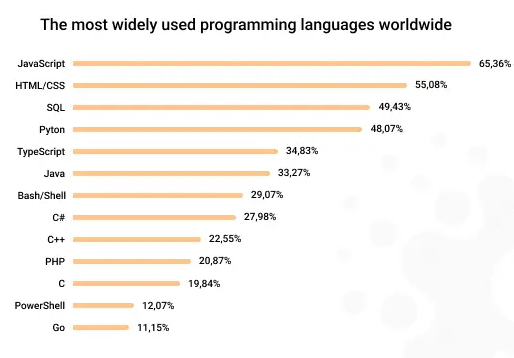
\includegraphics{images/top.png}
	\end{center}
	\fonte{stackoverflow}
\end{figure}
% ----------------------------------------------------------

\subsection{Expo}
O Expo é uma plataforma que simplifica o desenvolvimento de aplicativos móveis usando JavaScript e React Native. Com recursos nativos do dispositivo acessíveis e facilitando a colaboração e distribuição de aplicativos, o Expo oferece uma solução abrangente para criar aplicativos móveis.

Segundo (\textcite{Hugo}) o uso do Expo proporciona uma camada de abstração superior ao React Native, resultando em uma experiência aprimorada no desenvolvimento de software. Com o aumento do 
número de usuários de smartphones, especialmente nas plataformas Android e iOS, a necessidade de criar aplicativos para ambas as plataformas se tornou cada vez mais 
evidente. Nesse contexto, o Expo oferece uma vantagem no desenvolvimento híbrido, simplificando o processo de criação de aplicativos multiplataforma.


\begin{figure}[htb]
	\caption{\label{fig:Fig_1}Expo vantagens}
	\begin{center}
		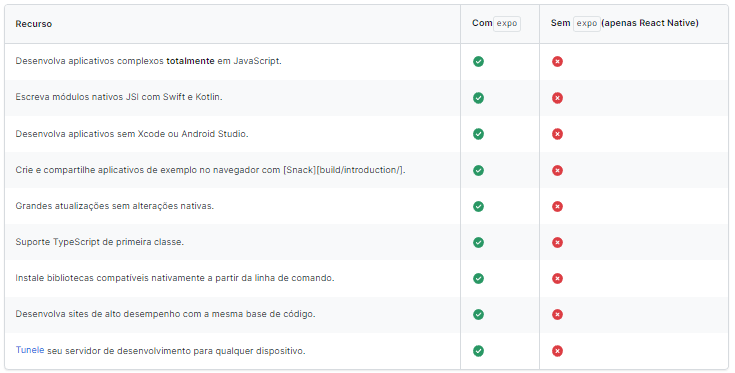
\includegraphics{images/expo.png}
	\end{center}
	\fonte{Expo}
\end{figure}

\subsection{Gin}
O framework Gin é uma biblioteca leve e rápida para construção de APIs em Go. Ele se baseia nos princípios do roteamento HTTP e fornece recursos poderosos para o desenvolvimento de aplicativos web escaláveis e de alto desempenho.

Ao utilizar o Gin, os desenvolvedores se beneficiam de uma sintaxe concisa e intuitiva, o que torna a criação de endpoints mais eficiente e produtiva. O framework oferece um roteamento flexível, permitindo mapear os diferentes endpoints para as funções correspondentes de forma clara e organizada.

Além disso, o Gin oferece suporte para a manipulação de parâmetros nas requisições HTTP. Isso permite que os desenvolvedores acessem e processem os dados enviados pelos clientes de forma simples e segura. O framework também oferece recursos para validação de entrada de dados, facilitando a verificação de formatos, tipos e restrições específicas, garantindo a integridade dos dados recebidos.

Outro aspecto importante do Gin é a sua eficiência e desempenho. Ele foi projetado para ser leve e rápido, proporcionando um processamento ágil das requisições. Isso é especialmente relevante em aplicações de grande escala, onde a capacidade de resposta e o tempo de processamento são cruciais.

O framework Gin também oferece recursos avançados, como middleware, que permite adicionar funcionalidades extras às rotas e endpoints da API. Isso inclui autenticação, autorização, logging e muitos outros aspectos que são essenciais para o desenvolvimento de sistemas seguros e escaláveis.

Em resumo, o uso do framework Gin proporciona uma base sólida e eficiente para o desenvolvimento de APIs RESTful. Sua sintaxe concisa, roteamento flexível, manipulação de parâmetros, validação de entrada e recursos avançados garantem a criação de endpoints robustos, escaláveis e de alto desempenho, possibilitando a construção de aplicações web modernas e eficientes.
